% ==============================================================================
% CHAPTER 3: TAXONOMY OF MULTI-AGENT COLLABORATIVE QA ARCHITECTURES
% ==============================================================================
\section{Taxonomy of Multi-Agent Collaborative QA Architectures}
\label{sec:taxonomy}

This review classifies a collaborative QA system primarily by the distribution
of \emph{decision authority and control}. The classification  is based on the
workflow that routes subtasks, determines when an answer is accepted, and
controls final synthesis. A \textbf{flat} architecture has no persistent agent with top-down
authority over the other participants. A \textbf{hierarchical} architecture
assigns planning, routing, approval, or synthesis authority to one or more
managers, or imposes an ordered, asymmetric control flow across stages. A
\textbf{hybrid} architecture changes this authority structure across task
stages or decision states.  Other design considerations such as communication topology (for example, broadcast, peer exchange, or a graph),
role specialization, human-in-the-loop (HITL) checkpoints, and runtime routing are orthogonal attributes. For example, a group-chat framework is
not automatically flat, and a system with specialized roles is not automatically
hierarchical. The three classes are alternative control patterns rather than
stages of a historical progression. 
Figure~\ref{fig:topology}
provides an illustrative schematic.

\begin{figure*}[pos=t]
	\centering
	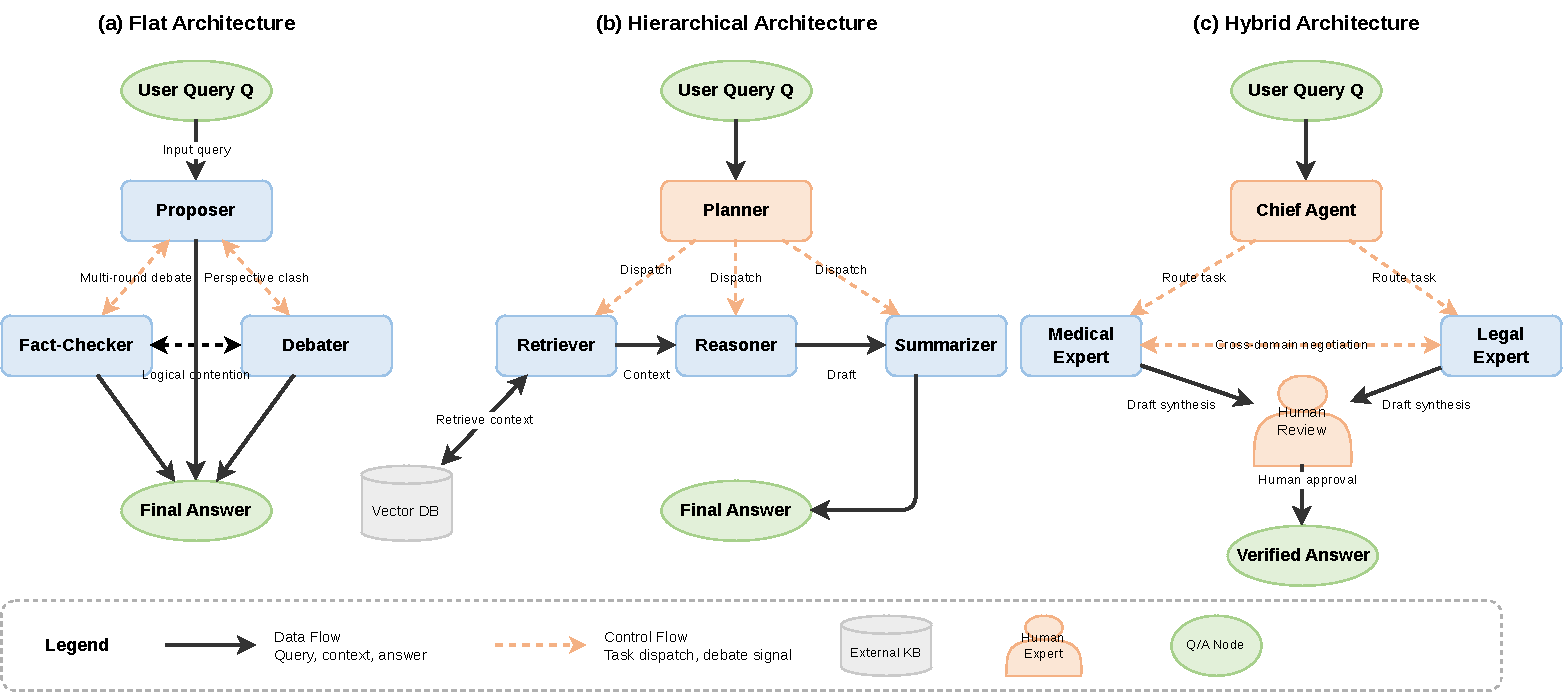
\includegraphics[width=\textwidth]{fig3_topology.pdf}
	\caption{Illustrative network topologies for multi-agent collaborative QA.
		The operational taxonomy is defined by decision authority and
		control, as specified in the text and Table~\ref{tab:core_taxonomy_mapping}.}
	\label{fig:topology}
\end{figure*}




\subsection{Flat Architectures}
\label{sec:flat}

In a flat collaborative architecture, participating agents exchange information, critique candidate solutions, or engage in negotiations without a persistent top-down controller. The relevant characteristic lies in distributed decision-making authority, rather than unrestricted dialogue. A flat workflow may still enforce turn limits, adopt voting rules, or include a designated final aggregation step.

\subsubsection{Multi-Agent Debate}
\label{sec:debate}

In the multi-agent debate paradigm, several LLM agents generate candidate answers and critique one another across one or more rounds. \citet{du2024multiagent_debate} report improved factuality and reasoning performance on the tasks they evaluate. Subsequent studies further identify the boundary conditions of this effect: divergent prompting can mitigate convergence toward similar reasoning paths \citep{liang2024divergent_debate}, while answer consistency and degeneration remain notable failure modes \citep{xiong2023inter_consistency}. ReConcile integrates heterogeneous models with confidence-weighted consensus \citep{chen2024reconcile}. Accordingly, adding more agents or debate rounds does not reliably boost QA performance; instead, the interaction rules, diversity of evidence, and aggregation procedure determine whether disagreement yields correction, inconsistency, or unnecessary computational cost.

\subsubsection{Role-Conditioned Collaboration}
\label{sec:roleplay}

Role-conditioned collaboration assigns different prompts or task views to participating agents. CAMEL \citep{li2023camel} employs an “AI User” and an “AI Assistant” paired with inception prompting to maintain role-conditioned interaction. This constitutes an adjacent multi-agent framework and does not serve as direct evidence that role playing improves QA accuracy. Within this taxonomy, role assignment is treated as an orthogonal attribute: the framework remains flat when no single role persistently controls task routing or final acceptance.

\subsubsection{Group-Chat Collaboration}
\label{sec:groupchat}

Group-chat collaboration adopts multi-participant conversations as its interaction interface. AutoGen \citep{wu2024autogen} supports developer-defined speaker selection rules and conversation patterns instead of enforcing a fully flat, free-form group chat paradigm. Accordingly, its resulting topology is determined by application configurations. It is best regarded as a technical framework capable of implementing flat, hierarchical, or hybrid workflows, rather than direct QA evidence.

Flat architectures can be useful when independent viewpoints, mutual critique, or open-ended exploration are required. Their distributed structure can reduce reliance on a single reasoning path, yet it also incurs coordination costs.
In fully connected settings, the number of potential communication links grows quadratically with the number of agents. Additional rounds may introduce redundant context, delayed convergence, correlated errors, or pseudo-consensus.
By contrast, when tasks demand stable dependencies, predictable execution, or stringent cost control, explicit authority and routing mechanisms may be more appropriate.

\subsection{Hierarchical Architectures}
\label{sec:hierarchical}

Hierarchical architectures delegate the authority for planning, routing, approval, or synthesis to one or more agents. Lower-level agents execute bounded subtasks or provide evidence to a manager. The workflow may take the form of a tree, a pipeline, or a controller–worker loop; its defining characteristic is asymmetric decision-making authority.

\subsubsection{Manager--Executor Pattern}
\label{sec:manager_executor}

The manager–executor pattern separates global planning from local execution.
MetaGPT \citep{hong2024metagpt} adopts standard operating procedures and defines roles
including product manager, architect, and engineer. ChatDev \citep{qian2023chatdev}
simulates a software development organisation via ChatChain. Both fall under related software engineering systems; they demonstrate structured delegation
yet do not provide direct evidence regarding QA performance. Their inclusion here
is therefore explanatory rather than comparative.

\subsubsection{Plan--Retrieve--Generate Pipeline}
\label{sec:pipeline}

Knowledge-intensive QA can assign planning, retrieval, generation, and
verification to a staged workflow. LONGAGENT \citep{zhao2024longagent}
coordinates a leader with document-reading members, Chain-of-Agents
\citep{zhang2024chain_agents} propagates information across context segments
before synthesis, and CoCoA \citep{jiang2026cocoa} coordinates parametric and
retrieved knowledge for QA. These role-I systems differ in their communication
and aggregation mechanisms, but each places subtask sequencing or synthesis
under explicit control. By contrast, HuggingGPT \citep{shen2024hugginggpt}
uses a controller to invoke specialised models and tools. It is retained as an
adjacent orchestration example, rather than as an autonomous multi-agent QA
architecture equivalent to the empirical QA studies.




Hierarchical architectures can improve controllability by separating global planning from local execution. They are suitable for QA workflows with stable procedures, explicit dependencies, or quality-control checkpoints. However, this centralisation may introduce a planner bottleneck: an erroneous high-level plan can propagate errors, and rigid pipelines may fail to handle unexpected evidence or conflicting expert opinions. Therefore, the associated benefits depend on the quality of the controller and the availability of corrective pathways.

\subsection{Hybrid Architectures}
\label{sec:hybrid}

Hybrid architectures alter the control configuration across task stages or decision states. A system may adopt peer deliberation to explore candidate solutions, hierarchical delegation to execute a selected plan, and conditional human oversight in scenarios where uncertainty or risk exceeds a predefined threshold. Simply combining individual components is insufficient; the coordination paradigm itself must be adaptive.

\subsubsection{Graph-Structured Agent Networks}
\label{sec:graph}

Graph-structured networks represent agents and transitions as an executable graph. LangGraph \citep{langgraph2024} serves as an official technical framework for defining state transitions, loops, and conditional branches; it provides technical evidence (role T), rather than constituting a QA evaluation. GPTSwarm \citep{zhuge2024gptswarm} is an empirical study of agent methodologies that optimises prompts and inter-agent graph connections. These sources carry distinct evidentiary roles and should not be treated as interchangeable demonstrations of QA effectiveness.

\subsubsection{Adaptive Collaboration-Mode Switching}
\label{sec:adaptive}

Adaptive systems adjust team composition or control patterns as tasks evolve.
AgentVerse \citep{chen2024agentverse} describes an iterative pipeline consisting of
expert recruitment, collaborative decision-making, action execution, and
result evaluation. This mechanism cannot be simplified to a ``simple-flat/complex-
hierarchical'' rule. MDAgents \citep{kim2024mdagents} provides direct
in-case evidence for adaptive medical collaboration. Such adaptive mechanisms
enhance routing flexibility, yet introduce extra requirements for state management
and performance evaluation.

\subsubsection{Human-in-the-Loop Design Pattern}
\label{sec:hitl}

The frameworks can pause at defined breakpoints for human review
\citep{langgraph2024}, which may be useful for high-risk decisions. However,
the present core corpus does not provide a matched empirical evaluation that
isolates the effect of such intervention in high-risk QA. Claims about safer or
more traceable decisions should therefore be framed as a design objective, not
an established performance result.



Hybrid architectures are useful when task requirements are heterogeneous or when the workflow must combine deliberation, controlled execution, and conditional review. Their trade-off lies in engineering complexity: dynamic routing, state transitions, and cross-mode information transfer are more difficult to configure, debug, evaluate, and reproduce. A hybrid design is justified when this additional adaptability addresses documented uncertainty or risk, rather than serving as a default replacement for fixed control patterns.

\subsection{Discussions}
\label{sec:arch_comparison}

Table~\ref{tab:9categories} compares the differences among various architecture types. 

\begin{table*}[pos=t]
  \centering
  \caption{Multi-agent Collaborative QA System Architecture}
  \label{tab:9categories}
  \scriptsize
  \begin{tabular}{p{1.4cm} p{2.0cm} p{2.4cm}  p{3.2cm} p{2.3cm} p{2.2cm}}
    \toprule
    \textbf{Architectures} & \textbf{Sub-category} & \textbf{Representative Studies} &
   \textbf{Control mechanism} &
    \textbf{Suitable conditions} & \textbf{ Limitations} \\
    \midrule
    \multirow{3}{*}{\textbf{Flat}} &
    Multi-party debate & \citet{du2024multiagent_debate} & 
    Peer critique and aggregation can add independent answer paths &
    Tasks needing competing factual or reasoning views &
    Cost, degeneration, and aggregation sensitivity \\
    & Role-conditioned interaction & CAMEL \citep{li2023camel} & 
    Personas structure interaction but do not by themselves establish QA gains &
    Exploratory collaboration and prompt-role studies &
    Fixed roles or correlated perspectives \\
    & Configurable group chat & AutoGen \citep{wu2024autogen}  &
    Developer-defined speaker selection and dialogue patterns &
    Applications requiring configurable conversations &
    Topology and QA performance depend on configuration \\
    \midrule
    \multirow{3}{*}{\textbf{Hierarchical}} &
    Manager--executor & MetaGPT \citep{hong2024metagpt}  &
    Manager assigns staged work to specialised executors &
    Structured engineering workflows &
    Planner bottleneck and error propagation \\
    & Controlled QA pipeline & LONGAGENT; Chain-of-Agents; CoCoA
    \citep{zhao2024longagent,zhang2024chain_agents,jiang2026cocoa}  &
    Explicit sequencing and final synthesis over distributed evidence &
    Long-document or knowledge-intensive QA &
    Information loss and coordination cost at synthesis \\
   
    \midrule
    \multirow{3}{*}{\textbf{Hybrid}} &
    Graph-routed network & GPTSwarm; LangGraph
    \citep{zhuge2024gptswarm,langgraph2024}  &
    Graph transitions permit loops, branches, and routing policies &
    Workflows with conditional state transitions &
    Different evidence roles; difficult debugging and tracing \\
    & Adaptive mode switching & MDAgents \citep{kim2024mdagents}  &
    Changes collaboration in response to case characteristics &
    Tasks with heterogeneous requirements &
    Routing policy must be evaluated, not assumed beneficial \\
    & HITL checkpoints & LangGraph breakpoints \citep{langgraph2024} &
    Human review at explicitly defined decision points &
    High-risk workflows requiring accountability &
    Direct comparative QA evidence remains limited \\
    \bottomrule
  \end{tabular}
\end{table*}

These architecture types differ in where decision authority is placed and when it
changes. Communication topology remains a useful secondary descriptor, but it
does not supersede the operational rules above. 
